In this section, we show how to extend the game-semantic correspondence
established for the $\lambda$-calculus to other languages such as \pcf\ and \ialgol.

\subsection{\pcf\ fragment}

The $Y$ combinator needs a special treatment. In order to deal with
it, we follow the idea of \cite{abramsky:game-semantics-tutorial}:
we consider the sublanguage $\pcf_1$ of \pcf\ in which the only
allowed use of the $Y$ combinator is in terms of the form $Y(
\lambda x:A .x )$ for some type $A$. We will write $\Omega_A$ to
denote the non-terminating term $Y(\lambda x:A .x)$ for a given type
$A$.

We introduce the \emph{syntactic approximants} to $Y_A M$:
\begin{eqnarray*}
Y^0_A M &=& \Gamma \vdash \Omega_A : A\\
Y^{n+1}_A M &=& M( Y^n M )
\end{eqnarray*}
For any \pcf\ term $M$ and natural number $n$, we define $M_n$ to be
the $\pcf_1$ term obtained from $M$ by replacing each subterm of the
form $Y N$ with $Y^n N_n$. We have $\sem{M} = \Union_{n\in\omega}
\sem{M_n}$ (\cite{abramsky:game-semantics-tutorial}, lemma 16).


\subsubsection{Computation tree}

We would like to define a unique computation tree for terms that use
the $Y$ combinator.

Let us first define the computation tree for $\pcf_1$ terms. We
introduce a special $\Sigma$-constant $\bot$ representing the
non-terminating computation of ground type $\Omega_o$. Given any
type $A = (A_1, \ldots, A_n, o)$, the computation tree
$\tau(\Omega_A)$ is defined to be the tree representation of
$\lambda x_1:A_1 \ldots x_n:A_n . \bot$. The computation tree of a
$\pcf_1$ term is then computed inductively in the standard way.

We now introduce a partial order on the set of computation trees.

A \emph{tree} $t$ is a labelling function $t:T\rightarrow L$ where
$T$, called the domain of $t$ and written $dom(t)$, is a non-empty
prefix-closed subset of some free monoid $X^*$ and $L$ denotes the
set of possible labels. Intuitively, $T$ represents the structure of
the tree (the set of all paths) and $t$ is the labelling function
mapping paths to labels. Trees can be ordered using the
\emph{approximation ordering} defined in \cite{KNU02}, section 1: we
write $t' \sqsubseteq t$ if the tree $t'$ is obtained from $t$ by
replacing some of its subtrees by $\bot$. Formally:
$$t' \sqsubseteq t \quad \iff dom(t') \subseteq dom(t) \wedge \forall  w \in dom(t'). (t'(w) = t(w) \vee t'(w) = \bot).$$
The set of all trees together with the approximation ordering is a
complete partial order.

We now consider a strict subset of the set of all trees: the set of
computation trees. A computation tree is a tree which represents the
$\eta$-normal form of some (potentially infinite) \pcf\ term. In
other words a tree is a computation tree if it can be written
$\tau(M)$ for some infinite \pcf\ term $M$. The set $L$ of labels is
constituted of the $\Sigma$-constants, @, the special constant
$\bot$, variables and abstractions of any sequence of variables. We
will write $(CT, \sqsubseteq)$ to denote the set of computation
trees ordered by the approximation ordering $\sqsubseteq$ defined
above. $(CT, \sqsubseteq)$ is also a complete partial order.

It is easy to check that the sequence of computation trees
$(\tau(M_n))_{n\in\omega}$ is a chain. We can therefore define the
computation tree of a \pcf\ term $M$ to be the least upper-bound of
the chain of computation trees of its approximants:
$$\tau(M) = \Union_{n\in\omega}(\tau(M_n))_{n\in\omega}.$$

In other words, we construct the computation tree by expanding
infinitely any subterm of the form $Y M$. For instance consider the
term $M = Y (\lambda f x. f x)$ where $f:(o,o)$ and $x:o$. Its
computation tree $\tau(M)$, represented below, is a tree
representation of the $\eta$-normal form of the infinite term
$(\lambda f x. f x) ((\lambda f x. f x) ((\lambda f x. f x)  (
\ldots$.
$$\tau(M) =
\begin{tikzpicture}[level distance=7mm,inner ysep=0.5mm,baseline=(root.base)]
\node (root) {$\lambda y$}
child {
    node {@}
    child {
        node {$\lambda f x$}
        child{
            node{$f$}
            child{
                node{$\lambda$}
                child{
                    node{$x$}
                }
            }
        }
    }
    child{
        node{$\tau(M)$}
    }
    child{
        node{$\lambda$}
        child{
            node{$y$}
        }
    }
};
\end{tikzpicture}
$$
The remaining operators of \ialgol\ are treated as standard
constants and the corresponding computation tree is constructed from
the $\eta$-normal form of the term in the standard way. For instance
the diagram below shows the computation tree for $\pcfcond\ b\ x\ y$
(left) and $\lambda x . 5$ (right):
$$\begin{tikzpicture}[level distance=7mm,inner ysep=0.5mm,baseline=(root.base)]
\path
node (root) {$\lambda b x y$}
child {
    node {\pcfcond}
    child {
        node {$\lambda$}
        child{
            node{$b$}
        }
    }
    child{
        node {$\lambda$}
        child{
            node{$x$}
        }
    }
    child{
        node {$\lambda$}
        child{
            node{$y$}
        }
    }
}
+(4,0)
node {$\lambda$}
child{
    node{$5$}
};
\end{tikzpicture}
$$
The node labelled $5$ has, like any other node, children
value-leaves which are not represented on the diagram above for
simplicity.

\subsubsection{Traversal}

New traversal rules accompany the additional constants of \ialgol.
There is one additional rule for natural number constants:
\begin{itemize}
\item \rulenamet{Nat} If $t \cdot n$ is a traversal where $n$ denotes a node labelled with some numeral constant $i\in \nat$ then
            $\Pstr{t \cdot (n){n} \cdot (in-n){i_n}}$
            is also a traversal where $i_n$ denotes the value-leaf of $m$ corresponding to the value $i\in \nat$.
\end{itemize}

\noindent The traversals rules for \pcfpred\ and \pcfsucc\ are
defined similarly. For instance, the rules for \pcfsucc\ are:
\begin{itemize}
\item \rulenamet{Succ} If $t \cdot \pcfsucc$ is a traversal and $\lambda$ denotes the only child node of \pcfsucc\ then
$\Pstr{t \cdot (succ){\pcfsucc} \cdot (l-succ,35:1){\lambda}}$ is also a traversal.

\item \rulenamet{Succ'} If
$\Pstr{ t_1 \cdot (succ){\pcfsucc} \cdot (l-succ,35:1){\lambda} \cdot t_2
\cdot (lv-l){i_{\lambda}}} $ is a traversal for some
$i \in \nat$ then $\Pstr{t_1 \cdot (succ){\pcfsucc} \cdot
(l-succ,35:1){\lambda} \cdot t_2 \cdot (lv-l){i_{\lambda}} \cdot
(succv-succ,25){(i+1)_{\pcfsucc}}}$ is also a traversal.
\end{itemize}

\noindent In the computation tree, nodes labelled with \pcfcond\
have three children nodes numbered from $1$ to $3$ corresponding to
the three parameters of the operator \pcfcond. The traversal rules
are:
\begin{itemize}
\item \rulenamet{Cond\mbox{-}If} If $t_1 \cdot \pcfcond$ is a traversal and $\lambda$ denotes the first child of \pcfcond\ then
$\Pstr{ t_1 \cdot (cond){{\pcfcond}} \cdot (l-cond,30:1){\lambda}}$
 is also a traversal.

\item \rulenamet{Cond\mbox{-}ThenElse} If
$\Pstr{t_1 \cdot (cond){\pcfcond} \cdot (l-cond,35:1){\lambda} \cdot t_2
\cdot (lv-l){i_{\lambda}}} $
then $\Pstr{t_1 \cdot
(cond){\pcfcond} \cdot (l-cond,35:1){\lambda} \cdot t_2 \cdot
(lv-l){i_{\lambda}} \cdot (condthenelse-cond,35:{2+[i>0]}){\lambda} }
$
is also a traversal. 



\item \rulenamet{Cond'} If
$\Pstr{t_1 \cdot (cond){\pcfcond} \cdot t_2 \cdot (l-cond,35:k){\lambda}
\cdot t_3 \cdot (lv-l){i_{\lambda}}}$
 for $k=2$ or $k=3$ then  $\Pstr{ t_1 \cdot
(cond){\pcfcond} \cdot t_2 \cdot (l-cond,35:k){\lambda} \cdot t_3
\cdot (lv-l){i_{\lambda}} \cdot (condv-cond,25){i_{\pcfcond}}}$
 is also a traversal.
\end{itemize}
It is easy to verify that these traversal rules are all
well-behaved. This completes the definition of traversal for the
\pcf\ subset of \ialgol.

\subsubsection{Interaction semantics}
We recall that the definition of the syntactically-revealed
semantics (Sec.\ \ref{sec:interaction_semantics}, Def.\
\ref{dfn:fully_revealed_semantics}) accounts for the presence of
interpreted constants: For any $\Sigma$-constant $f :
(A_1,\ldots,A_p,B)$ in the language, the revealed strategy of a term
of the form $\lambda \overline{\xi}. f N_1 \ldots N_p$ is defined
as:
$$ \revsem{\lambda \overline{\xi}. f N_1 \ldots N_p} = \langle \revsem{N_1}, \ldots, \revsem{N_p} \rangle \fatsemi^{0..p-1} \sem{f}.$$
where $\sem{f}$ is the standard strategy denotation of $f$.

\subsubsection{Correspondence theorem}
We would like to prove the counterpart of proposition
\ref{prop:rel_gamesem_trav} in the context of the simply-typed
$\lambda$-calculus \emph{with interpreted PCF constants}. The game
model of the language \pcf\ is given by the category $\mathcal{C}_b$
of well-bracketed strategies. Hence the well-bracketing assumption
stated at the beginning of section \ref{sec:gamesemcorresp} is
satisfied.

We first prove that $\travset(\_)^{\filter \theroot}$ is continuous.
\begin{lemma}
\label{lem:travred_continuous} Let $(S,\subseteq)$ denote the set of
sets of justified sequences of nodes ordered by subset inclusion.
The function $\travset(\_)^{\filter \theroot} : (CT,\sqsubseteq)
\rightarrow (S,\subseteq)$ is continuous.
\end{lemma}
\begin{proof} \
    \begin{description}
    \item[Monotonicity:] Let $T$ and $T'$ be two computation trees such that $T \sqsubseteq T'$
    and let $t$ be some traversal of $T$.
    Traversals ending with a node labelled $\bot$ are maximal therefore $\bot$ can only occur
    at the last position in a traversal. Let us prove the following two properties:
        \begin{itemize}
            \item[(i)]  If $t = t \cdot n$ with $n\neq \bot$ then $t$ is a traversal of $T'$;
            \item[(ii)] if $t= t_1 \cdot \bot$ then $t_1\in \travset(T')$.
        \end{itemize}

        (i) By induction on the length of $t$. It is trivial for the empty traversal.
            Suppose that $t = t_1 \cdot n$ is a traversal with $n \neq \bot$.
            By the induction hypothesis, $t_1$ is a traversal of $T'$.

            We observe that for all traversal rules, the traversal produced is of the form $t_1 \cdot n$ where
            $n$ is defined to be a child node or value-leaf of some node $m$ occurring in $t_1$.
            Moreover, the choice of the node $n$ only depends on the traversal $t_1$
            (for the constant rules, this is guaranteed by assumption (WB)).

            Since $T \sqsubseteq T'$, any node $m$ occurring in $t_1$ belongs
            to $T'$ and the children nodes and leaves of $m$ in $T$ also belong to the tree $T'$.
            Hence $n$ is also present in $T'$ and the rule used to produce the traversal $t$ of $T$
            can be used to produce the traversal $t$ of $T'$.

        (ii) $\bot$ can only occur at the last position in a traversal
        therefore $t_1$ does not end with $\bot$ and by (i) we have $t_1\in \travset(T')$.
\vspace{6pt}

        Hence we have:
        \begin{align*}
        \travset(T)^{\filter \theroot} &= \{ t \filter r \ | \ t \in \travset(T)     \} \\
        & = \{ (t\cdot n) \filter r \ | \ t\cdot n \in \travset(T) \wedge n \neq \bot \}
            \union \{ (t \cdot \bot ) \filter r \ | \ t \cdot \bot \in \travset(T)  \} \\
\mbox{(by (i) and (ii))} \quad        & \subseteq  \{ (t\cdot n)
\filter r \ | \ t\cdot n \in \travset(T') \wedge n \neq \bot
\}
            \union \{ t \filter r \ | \ t \in \travset(T')  \} \\
        & = \travset(T')^{\filter \theroot}
        \end{align*}

        \item[Continuity:] Let $t \in \travset \left( \Union_{n\in\omega} T_n \right)$.
        We write $t_i$ for the finite prefix of $t$ of length $i$.
        The set of traversals is prefix-closed therefore $t_i \in \travset \left( \Union_{n\in\omega} T_n \right)$ for any $i$.
        Since $t_i$ has finite length we have $t_i \in \travset(T_{j_i})$ for some $j_i \in \omega$.
        Therefore we have:
        \begin{align*}
          t \filter r &= (\bigvee_{i\in\omega} t_i ) \filter r   & (\mbox{the sequence $(t_i)_{i\in\omega}$ converges to $t$}) \\
          &= \Union_{i\in\omega} ( t_i \filter r )   & (\_ \filter r \mbox{ is continuous, lemma \ref{lem:projection_continuous}}) \\
          &\in \Union_{i\in\omega} \travset(T_{j_i})^{\filter \theroot}   & (t_i \in \travset(T_{j_i})) \\
          &\subseteq \Union_{i\in\omega} \travset(T_i)^{\filter \theroot}   & (\mbox{since } \{ j_i \sthat i \in \omega \} \subseteq \omega)
        \end{align*}

        Hence $\travset(\Union_{n\in\omega} T_n )^{\filter
        \theroot} \subseteq \Union_{n\in\omega}
        \travset(T_n)^{\filter \theroot}.$

    \end{description}
\end{proof}

\begin{proposition}
Let $\Gamma \vdash M : T$ be a PCF term and $r$ be the root of
$\tau(M)$. Then:
\begin{align*}
(i)  \quad\varphi_M(\travset(M)^*) = \revsem{M},  \\
(ii) \quad \varphi_M(\travset(M)^{\filter \theroot}) = \sem{M}.
\end{align*}
\end{proposition}
\begin{proof}
We first prove the result for $\pcf_1$: (i) The proof is an
induction identical to the proof of proposition
\ref{prop:rel_gamesem_trav}. However we need to complete the case
analysis with the $\Sigma$-constant cases:
\begin{itemize}
\item The cases \pcfsucc, \pcfpred, \pcfcond\ and numeral constants are straightforward.

\item Suppose $M = \Omega_o$ then $\travset(\Omega_o) = \prefset ( \{ \lambda \cdot \bot \} )$ therefore
$\travset(\Omega_o)^{\filter \theroot} = \prefset( \{ \lambda \}
)$ and $\sem{\Omega_o} = \prefset( \{ q \})$ with
$\varphi(\lambda) = q$. Hence $\sem{\Omega_o} = \varphi
(\travset(\Omega_o)^{\filter \theroot})$.
\end{itemize}
(ii) is a direct consequence of (i) and the Projection Lemma
\ref{lem:varphi_proj}. \vspace{10pt}

\noindent We now extend the result to \pcf. Let $M$ be a \pcf\ term,
we have:
\begin{align*}
\sem{M} &= \Union_{n\in\omega} \sem{M_n} & (\mbox{\cite{abramsky:game-semantics-tutorial}, lemma 16})\\
&= \Union_{n\in\omega} \travset(\tau(M_n))^{\filter \theroot} & (M_n \mbox{ is a $\pcf_1$ term}) \\
&= \travset(\Union_{n\in\omega} \tau(M_n) )^{\filter \theroot} & (\mbox{by continuity of $\travset(\_)^{\filter \theroot}$, lemma \ref{lem:travred_continuous}}) \\
&= \travset(\tau(M))^{\filter \theroot} & (\mbox{by definition of } \tau(M)) \\
&= \travset(M)^{\filter \theroot} & (\mbox{abbreviation}).
\end{align*}
\end{proof}

Hence by corollary \ref{cor:varphi_bij}, $\varphi$ defines a
bijection from $\travset(M)^{\filter \theroot}$ to $\sem{M}$:
$$\varphi : \travset(M)^{\filter \theroot} \stackrel{\cong}{\longrightarrow} \sem{M}.$$

\subsubsection{First example: the successor operator}

Consider the term $M = \pcfsucc\ 5$ whose computation tree is
represented below. The value-leaves are also represented on the
diagram, they are the vertices attached to their parent node with a dashed line.
\begin{center}
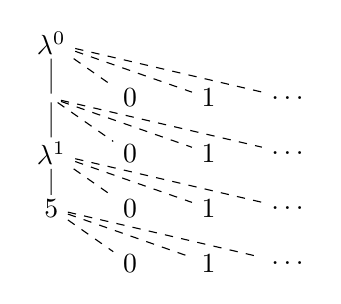
\begin{tikzpicture}[level distance=7mm,inner ysep=0.5mm,sibling distance=10mm]
\node {$\lambda^0$}
    child[missing]{}
    child[missing]{}
    child[missing]{}
    child {
        node {\pcfsucc}
        child[missing]{}
        child[missing]{}
        child[missing]{}
        child {
            node {$\lambda^1$}
            child[missing]{}
            child[missing]{}
            child[missing]{}
            child{
                node{$5$}
                child[missing]{}
                child[missing]{}
                child[missing]{}
                child[missing]{}
                child{node{$0$} edge from parent[dashed]}
                child{node{$1$} edge from parent[dashed]}
                child{node{$\ldots$} edge from parent[dashed]}
            }
            child{node{$0$} edge from parent[dashed]}
            child{node{$1$} edge from parent[dashed]}
            child{node{$\ldots$} edge from parent[dashed]}
        }
        child{node{$0$} edge from parent[dashed]}
        child{node{$1$} edge from parent[dashed]}
        child{node{$\ldots$} edge from parent[dashed]}
    }
    child{node{$0$} edge from parent[dashed]}
    child{node{$1$} edge from parent[dashed]}
    child{node{$\ldots$} edge from parent[dashed]}
;
\end{tikzpicture}
\end{center}

The following sequence of nodes is a traversal of $\tau(M)$:
$$ \Pstr[20pt]{ t = (l0){\lambda^0} \cdot (succ){\pcfsucc} \cdot (l1){\lambda^1} \cdot (c5){5} \cdot (v55-c5){5_5} \cdot (5l1-l1){5_{\lambda^1}} \cdot (6succ-succ){6_\pcfsucc} \cdot (6l0-l0,35){6_{\lambda^0}}}.
$$

The subsequences $t^*$ and $t \filter r$ are given by:
$$
\Pstr[17pt]{ t^* = (l0){\lambda^0} \cdot (l1-l0){\lambda^1} \cdot
(5l1-l1){5_{\lambda^1}} \cdot (6l0-l0){6_{\lambda^0}}.
\qquad  \mbox{ and } \qquad t
\filter r = (l0b){\lambda^0} \cdot
(6l0b-l0b){6_{\lambda^0}}. }
$$
We have $\varphi(t^*) = q_0 \cdot q_5 \cdot 5_{q_5} \cdot 5_{q_0}$
and $\varphi(t\filter r) = q_0 \cdot 5_{q_0}$ where $q_0$
and $q_5$ denote the roots of two flat arenas over $\nat$. These two
sequences of moves correspond to some play of the interaction
semantics and the standard semantics respectively. The interaction
play is represented below:
\begin{center}
\begin{tikzpicture}[style={anchor=base}]
\matrix (m) [matrix of math nodes]
{
\textbf{1} & \stackrel{5}{\longrightarrow} & \nat & \stackrel{\pcfsucc}{\longrightarrow} & \nat \\
&&&&  \node(q0){q_0}; \\
&&  \node(q5){q_5}; \\
&&  \node(a5){5_{q_5}}; \\
&&&&  \node(a6){6_{q_0}}; \\
};
\path (q5) edge[tableptr] (q0);
\draw[tableptr] (a5.west) .. controls +(160:0.2cm) and +(220:0.2cm) .. (q5.west);
\draw (a6) edge[tableptr] (q0);
\end{tikzpicture}
\end{center}

\subsubsection{Second example: the conditional operator}

\piccaption{The computation tree of the term $\lambda x y . \pcfcond\ 1\ x\ y$.}
\parpic[l]{
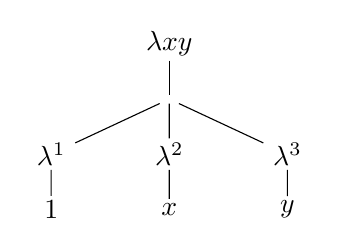
\begin{tikzpicture}[level distance=7mm,inner ysep=0.5mm,baseline=(root.base)]
\path
node (root) {$\lambda x y$}
child {
    node {\pcfcond}
    child {
        node {$\lambda^1$}
        child{
            node{$1$}
        }
    }
    child{
        node {$\lambda^2$}
        child{
            node{$x$}
        }
    }
    child{
        node {$\lambda^3$}
        child{
            node{$y$}
        }
    }
};
\end{tikzpicture}
}
Take the computation tree represented on the left (value-leaves are not shown). For any value $v \in\mathcal{D}$ the following sequence of nodes is a traversal:
$$\Pstr[27pt]{ t = (lxy){\lambda x y} \cdot (cond){\pcfcond} \cdot (l1-cond){\lambda^1} \cdot (1){1} \cdot (v11-1){1_1}
    \cdot (l3){\lambda^3} \cdot (y-lxy){y} \cdot (vy-y){v_y}  \cdot (vl3-l3){v_{\lambda^3}} \cdot (vcond-cond,30){v_{\pcfcond}}
    \cdot (vlxy-lxy,30){v_{\lambda x y}}.
}
$$
The subsequence $t^*$ and the reduction $t \filter\theroot$ are:
$$
\Pstr[17pt]{ t^* =  (lxy){\lambda x y} \cdot
        (l1-lxy){\lambda^1} \cdot
        (l3-lxy){\lambda^3} \cdot
        (y-lxy){y} \cdot
        (vy-y){v_y}  \cdot
        (vl3-l3){v_{\lambda^3}} \cdot
        (vlxy-lxy,35){v_{\lambda x y}}
\qquad  \mbox{ and } \qquad t \filter\theroot =
(lxyb){\lambda x y} \cdot (yb-lxyb){y} \cdot (vyb-yb){v_y}
\cdot (vlxyb-lxyb){v_{\lambda x y}}.
}
$$
The correspondence theorem tells us that the sequence of moves $\varphi(t^*)$ (represented in the diagram below) is a play of the
revealed semantics, and the sequence $\varphi(t\filter\theroot)$
is a play of the standard semantics that is obtained by hiding the internal moves from $\varphi(t^*)$.

\begin{center}
\begin{tikzpicture}[style={anchor=base}]
  \matrix[matrix of math nodes]
  {
  \nat & \times & \nat & \stackrel{\sigcol{\langle \sem{1}, \pi_1, \pi_2\rangle}}\longrightarrow & \nat & \times & \nat & \times &
\nat & \stackrel{\mucol\pcfcond}\longrightarrow & \nat \\
&&&&&&&&&&  \node(q0){q_0^{(\lambda x y)}}; \\
&&&&  \node(qa){q_a^{(\lambda^1)}}; \\
&&&&  \node(1){1}; \\
&&&&&&  \node(qb){q_b^{(\lambda^2)}}; \\
&&  \node(qy){q_y^{(y)}}; \\
&&  \node(vqy){v_{q_y}}; \\
&&&&&&  \node(vqb){v_{q_b}}; \\
&&&&&&&&&& \node(vq0){v_{q_0}}; \\
};
\path (vq0) edge[tableptr] (q0);
\path (vqb) edge[tableptr] (qb);
\draw[->] (vqy.west) .. controls +(160:0.2cm) and +(220:0.2cm) .. (qy.west);
\path (qy) edge[tableptr] (qb);
\path (qb) edge[tableptr] (q0);
\draw[->] (1.west) .. controls +(160:0.2cm) and +(200:0.2cm) .. (qa.west);
\path (qa) edge[tableptr] (q0);
\end{tikzpicture}
\end{center}


\subsection{Idealized algol}

We now consider the language Idealized Algol. The general idea is the same as for \pcf, however there are some difficulties caused by the presence of the two new
base types \iavar\ and \iacom. We just give indications on how to
adapt our framework to the particular case of \ialgol\ without
giving the complete proofs. However we believe that enough
indications are given to convince the reader that the argument used
in the \pcf\ case can be easily adapted to \ialgol.

\subsubsection{Computation hypertree}
Crucially, all the languages that we have considered up to now (lambda calculus and \pcf) do not have product types. Consequently, the arenas involved in their game model only have a single initial move at most, and therefore they can be
regarded as trees. This had permitted us to represent the game denotation of term directly on some representation of its abstract syntax tree. In \ialgol, however, the type \iavar\ is given by the product $\iacom^{\nat} \times \iaexp$. Therefore the corresponding game has an infinite number of initial moves. But tree structures such as the AST of the term have only one root therefore we have to find a different way to represent the game semantics.

The solution consists in using a hypertree representation instead of just a tree. This hypertree is an abstract graph representation of the syntax of the term in which some nodes, called \emph{generalized lambda nodes}, are themselves constituted of (possibly infinitely many) subnodes. Each subnode can be connected to different children nodes of the generalized node.


\emph{Notations:} For any type $\mu$, we write
$\mathcal{D}_\mu$ to denote the set of values of type $\mu$.
We have $\mathcal{D}_{\iaexp} = \nat$,
$\mathcal{D}_{\iacom} = \{ \iadone \}$
and $\mathcal{D}_{\iavar} = \mathcal{D}_{\iaexp} \union \mathcal{D}_{\iacom}$. For any node $n$, if $\kappa(n)$ is of type $(A_1,\ldots A_n,B)$, we call $B$ the \emph{return type of $n$}. The set of value-leaves of a node $n$ is given by $\mathcal{D}_{\mu}$ where $\mu$ is the return type of $n$.
For conciseness, when representing value-leaves in the DAG, we merge all the value-leaves of a given node of type $\mu$ into a single leaf labelled $\mathcal{D}_\mu$.

For instance the tree
\begin{center}
\begin{tikzpicture}[level distance=7mm,inner ysep=0.5mm,baseline=(root.base),sibling distance=5mm]
\path
node (root) {$n$}
child {
    node {$\mathcal{D}_\iaexp$}
}
+(1.5,0) node {stands for}
+(3,0)
node {$n$}
    child {node {$0$} }
    child {node {$1$}}
    child {node {$2$}}
    child {node {$\ldots$}}
+(7,0) node {and}
+(8,0)
node {$n$}
child{
    node{$\mathcal{D}_\iacom$}
}
+(9,0) node {for}
+(10,0)
node {$n$}
child{
    node{\iadone}
};
\end{tikzpicture}.
\end{center}

The computation hypertree of a term of type \iavar has infinitely many root $\lambda$-nodes which are merged all-together into a single node called a \defname{generalized lambda-node}. Nodes with return type \iavar have a generalized lambda node as parent.
The subnodes of a generalized lambda nodes are labelled
$\lambda^r$, $\lambda^{w_0}$, $\lambda^{w_1}$, $\lambda^{w_2}$, \ldots
Suppose that $M$ is a term of type \iavar, then the computation hypertree for $\lambda \overline{\xi} . M$ is obtained by relabelling the root $\lambda$-nodes $\lambda^r$,
$\lambda^{w_0}$, $\lambda^{w_1}$, $\lambda^{w_2}$, \ldots into
$\lambda^r \overline{\xi}$, $\lambda^{w_0} \overline{\xi}$,
$\lambda^{w_1} \overline{\xi}$, $\lambda^{w_2} \overline{\xi}$,
\ldots. For a term $M$  of type \iaexp\ or \iacom, the computation
hypertree for $\lambda \overline{\xi} . M$ is computed as defined previously for computation trees in the $\lambda$-calculus.

Table \ref{tab:ia_computationdag} shows the computation hypertree for each term-construct of \ialgol. The generalized lambda nodes are circled (line 2 and 6).

\notetoself{circle the gener. lambda nodes}

\begin{table}
\begin{center}
\begin{tabular}{lc}
$M$ & $\tau(M)$ \\ \hline \hline \\
\parbox{3cm}{x $: \mu$ \\
$\mu \in \{ \iacom, \iaexp \}$} &

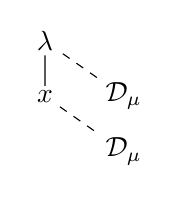
\begin{tikzpicture}[level distance=7mm,inner ysep=0.5mm,sibling distance=10mm]
\node {$\lambda$}
child[missing]{}
child {
    node {$x$}
    child[missing]{}
    child[missing]{}
    child {
        node {$\mathcal{D}_\mu$}
        edge from parent[dashed]
    }
}
child{node{$\mathcal{D}_\mu$} edge from parent[dashed]}
;
\end{tikzpicture}
\\ \\
x : \iavar &
\begin{tikzpicture}
\matrix (m) [matrix of math nodes, row sep=5mm]
{
\lambda^r & \lambda^{w_0} & \lambda^{w_1}  & \lambda^{w_2} & \lambda^{w_{\ldots}} \\
    \mathcal{D}_\iaexp &  & x & & \iadone \\
    &  &  & \mathcal{D}_\iaexp & \iadone \\
};
\draw[-] (m-1-1) -- (m-2-3)
         (m-1-2) -- (m-2-3)
         (m-1-3) -- (m-2-3)
         (m-1-4) -- (m-2-3)
         (m-1-5) -- (m-2-3);
\draw[dashed] (m-2-3) -- (m-3-4)
              (m-2-3) -- (m-3-5)
              (m-1-1) -- (m-2-1)
              (m-1-5) -- (m-2-5)
              (m-1-4) -- (m-2-5)
              (m-1-3) -- (m-2-5)
              (m-1-2) -- (m-2-5);
\end{tikzpicture}
\\ \\
\iaskip : \iacom &
    \begin{tikzpicture}[level distance=7mm,inner ysep=0.5mm,sibling distance=10mm]
\node {$\lambda$}
child[missing]{}
child {
    node {\iaskip}
    child[missing]{}
    child[missing]{}
    child {
        node {\iadone}
        edge from parent[dashed]
    }
}
child{node{\iadone} edge from parent[dashed]}
;
\end{tikzpicture}
\\ \\
$\iaassign\ L\ N :\iacom$ &
\begin{tikzpicture}[level distance=7mm,inner ysep=0.5mm,sibling distance=20mm]
\node {$\lambda$}
child[missing]{}
child {
    node {\iaassign}
    child{node{$\tau(N:\iaexp)$}}
    child{node{$\tau(L:\iavar)$}}
    child {
        node {\iadone}
        edge from parent[dashed]
    }
}
child{node{\iadone} edge from parent[dashed]};
\end{tikzpicture}
\\ \\
$\iaderef\ L :\iaexp$ &
\begin{tikzpicture}[level distance=7mm,inner ysep=0.5mm,sibling distance=15mm]
\node {$\lambda$}
child[missing]{}
child {
    node {\iaderef}
    child[missing]{}
    child{node{$\tau(L:\iavar)$}}
    child {
        node {\iadone}
        edge from parent[dashed]
    }
}
child{node{\iadone} edge from parent[dashed]}
;
\end{tikzpicture}
\\ \\
\parbox{3cm}{$\iaseq_{\mu}\ N_1\ N_2 :\iacom$\\ $\mu\in\{\iaexp,\iacom\}$} &
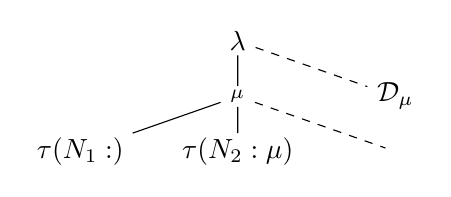
\begin{tikzpicture}[level distance=7mm,inner ysep=0.5mm,sibling distance=20mm]
\node {$\lambda$}
child[missing]{}
child {
    node {$\iaseq_\mu$}
    child{node{$\tau(N_1:\iacom)$}}
    child{node{$\tau(N_2:\mu)$}}
    child { node {\iadone} edge from parent[dashed] }
}
child{node{$\mathcal{D}_\mu$} edge from parent[dashed]};
\end{tikzpicture}
\\ \\
$\iamkvar\ N_w\ N_r :\iavar$ &
\begin{tikzpicture}
\matrix (m) [matrix of math nodes, row sep=5mm]
{
  \lambda^r & \lambda^{w_0} & \lambda^{w_1}  & \lambda^{w_2} & \lambda^{w_{\ldots}} \\
    \mathcal{D}_\iaexp &  & \iamkvar & & \iadone \\
    & \tau(N_r) & \tau(N_w) & \mathcal{D}_\iaexp & \iadone \\
};
\draw[-] (m-1-1) -- (m-2-3)
         (m-1-2) -- (m-2-3)
         (m-1-3) -- (m-2-3)
         (m-1-4) -- (m-2-3)
         (m-1-5) -- (m-2-3)
         (m-2-3) -- (m-3-2)
         (m-2-3) -- (m-3-3);
\draw[dashed] (m-2-3) -- (m-3-4)
              (m-2-3) -- (m-3-5)
              (m-1-1) -- (m-2-1)
              (m-1-5) -- (m-2-5)
              (m-1-4) -- (m-2-5)
              (m-1-3) -- (m-2-5)
              (m-1-2) -- (m-2-5);
\end{tikzpicture}
\\ \\
\parbox{3cm}{$\ianewin{x}\ N : \mu$ \\ $\mu \in \{ \iacom, \iaexp \} $} &
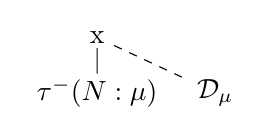
\begin{tikzpicture}[level distance=7mm,inner ysep=0.5mm,sibling distance=15mm]
\node {\ianewin{x}}
child[missing]{}
child{node{$\tau^-(N:\mu)$}}
child { node {$\mathcal{D}_\mu$} edge from parent[dashed]};
\end{tikzpicture}
\end{tabular}
\bigskip

where $\tau^-(N)$ denotes the DAG obtained by removing the root nodes from $\tau^-(N)$.
\end{center}
  \caption{Computation DAGs for the constructs of \ialgol.}
  \label{tab:ia_computationdag}
\end{table}

In a computation hypertree, the parent of a generalized lambda nodes shares an edge with each of the lambda node inside the generalized lambda node. Therefore in Table \ref{tab:ia_computationdag},

... stands for ...

\notetoself{ typset the corresponding trees}


\emph{Notation:} Let $p$ be a node and suppose that its $i$th child $n$ has the
return type \iavar. Then $n$ is a generalized lambda-node with subnodes
$\lambda^r \overline{\xi}$, $\lambda^{w_0}
\overline{\xi}$, \ldots. From the point of view of the parent node $p$, these nodes are referenced as ``$i.\alpha$'' where $i\in\{0..arity(p)\}$ and $\alpha \in \{ r\} \union\{ w_k \ | \ k \in \nat \}$. For instance  $i.r$ refers to the root labelled $\lambda^r \overline{\xi}$ of the $i$th child of $p$, and
$i.w_k$ refers to the root labelled $\lambda^{w_k} \overline{\xi}$.




\subsubsection{Traversals}


\begin{itemize}
\item \emph{The application rule}

There are two rules (app$_{\iaexp}$) and (app$_{\iacom}$)
corresponding to traversals ending with an @-node of return type
\iaexp\ and \iacom\ respectively. These rules are identical to the
rule \iaexp\ of section \ref{subsec:traversal}.

The application rule for $@$-nodes with return type \iavar\ is:
$$\rulename{app_\iavar}
\rulef{ \Pstr{t \cdot (lHyp){\lambda^k \overline{\xi}} \cdot
(appHyp-lHyp,35:0){@} \in \travset }
 }{\Pstr[18pt] {t \cdot (l){\lambda^k
\overline{\xi}} \cdot (app-l,35:0){@} \cdot (l2-app,35:0.k){\lambda^k
\overline{\eta}} \in \travset }}
 \ k \in \{ r, w_0, w_1, \ldots \}
$$


\item \emph{Input-variable rules}

There are two rules \rulenamet{InputVar^\iaexp} and \rulenamet{InputVar^\iacom}
which are the counterparts of rule \rulenamet{InputVar} of section
\ref{subsec:traversal} and are defined identically.

Let $x$ be an input-variable of type \iavar.
$$ \rulename{InputVar^\iavar_r}
\rulef{t \cdot \lambda^r \overline{\xi} \cdot x \in \travset \qquad v\in\mathcal{D} }
    {t \cdot \lambda^r \overline{\xi} \cdot \rnode{x}{x} \cdot v_x \in \travset}
\hspace{1.5cm} \rulename{InputVar^\iavar_w} \rulef{t \cdot
\lambda^{w_i} \overline{\xi} \cdot x \in \travset}
    {t \cdot \lambda^{w_i} \overline{\xi} \cdot \rnode{x}{x} \cdot \iadone_x \in \travset }
$$

\item \emph{IA constants rules}

Table \ref{tab:ia_travrules} gives the traversal rules corresponding to the interpreted constants of \ialgol.
The rules for \ianew\ are purely structural, they are defined the
same way as the rules \rulenamet{app_\iaexp}, \rulenamet{app_\iacom} and
\rulenamet{app_\iadone}.

\begin{table}[htbp]
$$
\begin{array}{ll}
\rulename{deref} \rulef{t \cdot \iaderef \in \travset}{\Pstr[15pt]{t \cdot (d){\iaderef} \cdot (n-d,35:1.r){n} \in \travset }}
&
\rulename{deref'}
\rulef{t \cdot \iaderef \cdot n \cdot t_2 \cdot v_n \in \travset} {t
\cdot \iaderef \cdot n \cdot t_2 \cdot v_n \cdot v_{\iaderef}\in
\travset }
\\[30pt]
\rulename{assign} \rulef{t \cdot \iaassign \in \travset}{\Pstr[16pt]{t \cdot (ass){\iaassign} \cdot (n-ass,35:1){\lambda} \in \travset} }
&
\rulename{assign'}
\rulef{\Pstr{t \cdot \iaassign \cdot (n)\lambda \cdot t_2 \cdot (vn-n){v_\lambda}} \in
\travset} {\Pstr[25pt]{t \cdot (ass){\iaassign} \cdot (n){\lambda} \cdot
t_2 \cdot (vn-n){v_\lambda} \cdot (m-ass,35:2.w_n){\lambda\overline\eta} \in \travset } }
\\[40pt]
\multicolumn{2}{l}{\rulename{assign''}  \rulef{\Pstr[1.7cm]{t \cdot (assHyp){\iaassign} \cdot t_2 \cdot (mHyp-assHyp,35:2.w_k){\lambda\overline\eta} \cdot t_3 \cdot (vmHyp-mHyp){\iadone_{\lambda\overline\eta}} \in \travset}}
{\Pstr[0.7cm]{t \cdot (ass)\iaassign \cdot t_2 \cdot (m){\lambda\overline\eta} \cdot t_3 \cdot (vm-m,25){\iadone_{\lambda\overline\eta}} \cdot
(vass-ass,20){\iadone_\iaassign} \in \travset} }
}
\\[30pt]
\rulename{seq} \rulef{t \cdot \iaseq \in \travset}{\Pstr[13pt]{t \cdot (seq){\iaseq} \cdot (n-seq,35:1){n} \in \travset } }
&
\rulename{seq'}
\rulef{t \cdot \iaseq \cdot n \cdot t_2 \cdot v_n \in
\travset} {\Pstr[18pt]{ t \cdot (seq){\iaseq} \cdot (n){n} \cdot t_2
\cdot v_n \cdot (m-seq,25:2){m} \in \travset }}
\\[30pt]
\multicolumn{2}{l}{\rulename{seq''} \rulef{\Pstr{t \cdot (seqHyp){\iaseq} \cdot t_2 \cdot (mHyp-seqHyp,35:2){m} \cdot t_3 \cdot v_m \in \travset}}
{t \cdot \iaseq \cdot t_2 \cdot m \cdot t_3 \cdot v_m \cdot
v_{\iaseq} \in \travset }}
\\[30pt]
\rulename{mkvar_r} \rulef{t \cdot \lambda^r \overline{\xi} \cdot \iamkvar \in \travset}{\Pstr[14pt]{t \cdot \lambda^r \overline{\xi} \cdot (d){\iamkvar} \cdot (n-d,35:1){\lambda} \in \travset} }
&\rulename{mkvar_r'}
\rulef{\Pstr{t \cdot \iamkvar \cdot (n)\lambda \cdot t_2 \cdot (vn-n){v_\lambda} \in \travset}} {\Pstr[17pt]{t \cdot (mk)\iamkvar \cdot (n)\lambda \cdot t_2 \cdot (vn-n){v_\lambda} \cdot (vmk-mk,25){v_{\iamkvar}}\in
\travset}}
\\[30pt]
\rulename{mkvar_w} \rulef{t \cdot \lambda^{w_k} \overline{\xi} \cdot \iamkvar \in \travset}{\Pstr[15pt]{t \cdot \lambda^{w_k} \overline{\xi} \cdot (mk){\iamkvar} \cdot (n-mk,35:2){\lambda\overline\eta} \in \travset} }
%\\[30pt] \multicolumn{2}{l}
&
{\rulename{mkvar_w''}  \rulef{\Pstr[25pt]{t \cdot \lambda^{w_k} \overline{\xi} \cdot \iamkvar \cdot (n){\lambda\overline\eta} \cdot t_2 \cdot (vn-n,25){\iadone_{\lambda\overline\eta}} \in \travset}}
{\Pstr[17pt]{t \cdot \lambda^{w_k} \overline{\xi} \cdot (mk)\iamkvar \cdot (n){\lambda\overline\eta} \cdot
t_2 \cdot (vn-n,25){\iadone_{\lambda\overline\eta}} \cdot (vmk-mk,20)\iadone_{\iamkvar} \in \travset}}
}
\end{array}
$$
where $v$ denotes some value from $\mathcal{D}$.
\caption{Traversal rules for \ialgol\ constants}
\label{tab:ia_travrules}
\end{table}


The four rules given in Table \ref{tab:ia_travrules} are not sufficient to model the constant \iamkvar.
Indeed, consider the term $\iaassign\ (\iamkvar\ (\lambda x . M) N)
7$. The rule (\mbox{mkvar}$_w''$) permits to traverse the node
\iamkvar\ and to go on by traversing the computation tree of
$\lambda x . M$. The problem is that when traversing $\tau(M)$, if
we reach a variable $x$, we are not able to relate $x$ to the value
$7$ that is assigned to the variable.

To overcome this problem, we need to define traversal rules for
variable in such a way that a variable node bound by the second
child of a $\iamkvar$-node is treated differently from other
variables.

\item \emph{Variable rules}
Let $x$ be an internal variable node \ie either hereditarily justified by an @-node or by a $\Sigma$-constant node. There are two cases depending on whether $x$ is a $\lambda$-abstracted variable or a block-allocated variable declared with a ``$\ianewin{x}$'' construct.

\begin{itemize}
\item Suppose that $x$'s binder is a lambda-node $\lambda \overline{x}$ and $x \in N^{@\vdash}$.

Then this occurrence of $x$ corresponds to an internal variable of type \iavar\ which would be substituted by another term if the term were to be reduced to normal form. This case is treated a generalization of the case treated by rule \rulenamet{Var} (see Sec.\ \ref{subsec:traversal}) to variables of type \iavar. This generalization is straightforward: the lambda nodes preceding $x$ in the traversals determines which lambda-nodes will be visited next:
$$ \rulename{Var_\iavar}
    \rulef{\Pstr[0.5cm]{t \cdot (n){n} \cdot (lx){\lambda \overline{x}}     \ldots \lambda^\alpha x_i \cdot (x-lx,50:i){x_i} } \in \travset \quad x_i \in N_{\sf var}^{@\vdash}}
{\Pstr[23pt]{t \cdot (n){n} \cdot (lx){\lambda \overline{x}}
\ldots \lambda^\alpha x_i \cdot  (x-lx,30:i){x_i} \cdot (letai-n,40:i.\alpha){\lambda\overline{\eta_i}}
\in \travset \raisebox{0pt}[25pt]{}}}
$$
where $\alpha$ belongs to $\{r\} \union \{w_i \ | \ i \in \nat \}$.

\item Suppose that $x$'s binder is a lambda-node and $x \in N^{N_\Sigma\vdash}$.

In \ialgol, the only $\Sigma$-constant node of order greater than 1 is \iamkvar, therefore a lambda-node that is hereditarily enabled by a $\Sigma$-node is necessarily the second child of a \iamkvar-node.
Hence $x$'s binder is a lambda node labelled $\lambda x$
and is the second child of a \iamkvar-node. This case is handled by the following rule:
$$ \rulename{\iamkvar\mbox{-}Var}  \rulef{\Pstr[17pt]{t \cdot \lambda^{w_k} \overline{\xi} \cdot \iamkvar \cdot (lx)\lambda x \cdot t_2 \cdot (x-lx)x \in \travset}}
{\Pstr[15pt]{t \cdot \lambda^{w_k}\overline{\xi} \cdot \iamkvar \cdot (lx)\lambda x \cdot t_2 \cdot (x-lx)x \cdot (kx-x)k_x \in \travset }}
$$

\item Suppose that $x$ is block-allocated with $\ianewin{x}$.

In a justified sequence of nodes of the form
$\Pstr[17pt]{(decl){\ianewin{x}}\cdot \ldots \cdot \lambda^{w_k}\overline\xi \cdot (x-decl,25){x}}$ for some $k\in \mathcal{D}_{\iaexp}$, the segment  $\lambda^{w_k}\overline\xi \cdot x$ is called an \defname{assignment of $x$ with respect to (the occurrence of)  the node ``\ianewin{x}''}. We have the following rules:
$$
\begin{array}{lll}
\rulename{\ianew\mbox{-}Var_w}
&
    \rulef{
        t \cdot \lambda^{w_k} \overline{\xi} \cdot x \in \travset
        \quad x \in N^{\ianew\vdash}_{\sf var}
    }
    {   t \cdot \lambda^{w_k} \overline{\xi} \cdot x \cdot \iadone_x \in
        \travset
    },
\\[20pt]
\rulename{\ianew\mbox{-}Var_r}
&
    \rulef{
        \Pstr[17pt]{t_1 \cdot (decl){\ianewin{x}} \cdot t_2 \cdot \lambda^r \overline{\xi} \cdot (x-decl,25){x} \in \travset}
    }
    {   t_1 \cdot \ianewin{x} \cdot t_2 \cdot \lambda^r \overline{\xi}
        \cdot x \cdot 0_x \in \travset
    }
&    \parbox{4cm}{if $t_2$ contains no assignment of $x$;}
\\[20pt]
\rulename{\ianew\mbox{-}Var'_r}
&    \rulef{
        \Pstr[15pt]{
            t_1 \cdot (decl){\ianewin{x}} \cdot t_2 \cdot \lambda^r \overline{\xi} \cdot (x-decl,25){x} \in \travset
        }
    }
    {
        t_1 \cdot \ianewin{x} \cdot t_2 \cdot \lambda^r \overline{\xi} \cdot x \cdot k_x \in \travset
    }
&    \parbox{4cm}{if the last assignment of $x$ in $t_2$ is
of the form $\lambda^{w_k} \cdot x$ for some $k\in\nat$.}
\end{array}$$
\end{itemize}
\end{itemize}

\subsubsection{Game semantics correspondence}
The properties that we proved for computation trees and traversals
of the $\lambda$-calculus with constants can easily be lifted
to computation hypertrees of \ialgol. In particular:
\begin{itemize}
\item constant traversal rules are well-behaved (for order-$0$ and order-$1$ constants, this is a consequence
of Lemma \ref{lem:sigma_order1_are_wellbehaved}; for $\iamkvar$
however it needs to be proved separately);
\item P-view of traversals are paths in the computation hypertrees;
\item the P-view of the reduction of a traversal is the reduction of the P-view,
and the O-view of a traversal is the O-view of its reduction
(Lemma \ref{lem:pview_trav_projection} and
\ref{lem:oview_trav_projection});
\item there is a mapping from vertices of the computation hypertrees to moves in the interaction game semantics;
\item there is a correspondence between traversals of the computation tree and plays in interaction game semantics;
\item consequently, there is a correspondence between the standard game semantics and
the set of justified sequences of nodes $\travset(M)^{\filter
\theroot}$.
\end{itemize}
